\input{../../../../.preambles/02-lab_work}
\input{../../../../.preambles/20-math}
\newgeometry{top=1.5cm, bottom=1.5cm, left=1cm, right=1cm}
\begin{document}
    \begin{table}[h!]
        \center
        \begin{tabular}{|C{.5}|C{.2}|C{.25}|}
            \hline
            \multicolumn{1}{|c|}{\multirow{4}{*}{Лабораторная работа № 3}} &
            Студент, группа & , Ф-469 \\ \cline{2-3}
            & Дата выполнения & 23.09.2013 \\ \cline{2-3}
            & Подпись &  \\ \cline{2-3}
            Исследование статических & Дата отчёта & \\ \cline{2-3}
            характеристик триода & Оценка &  \\ \cline{2-3}
            & Подпись &  \\ \hline
        \end{tabular}
    \end{table}

    \emph{Цель работы:} изучение методов определения статических характеристик
    триода и изучение режимов его работы.
    
    \begin{figure}[h!]
        \center
        \includegraphics[width=.45\textwidth]{appearance} \hspace*{2em}
        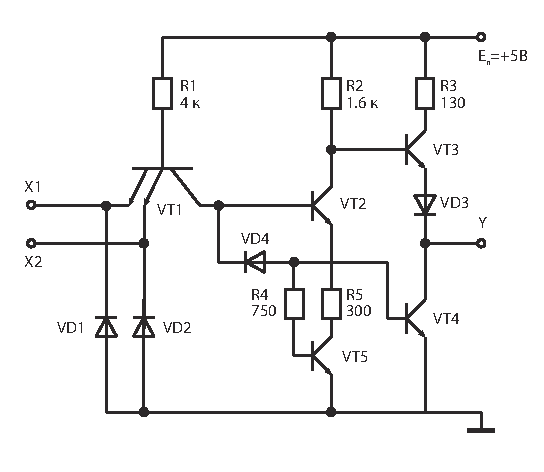
\includegraphics[width=.4\textwidth]{scheme}
        \parbox{.45\textwidth}{\caption{Внешний вид экспериментального макета}}
        \hspace*{2em}
        \parbox{.4\textwidth}{\caption{Принципиальная электрическая схема
        экспериментальной установки}}
    \end{figure}
    
    \begin{table}[h!]
        \center
        \caption{Семейство анодно-сеточных характеристик}
        % 50 75 100 125 150 175 200 220 235 250
        \begin{tabular}{|m{.1\textwidth}|*{11}{C{.05}|}} \hline
        \multirow{2}{*}{\( U_{a_{01}} = \)} &
            \( U_c \),~В &&&&&&&&&& \\ \cline{2-12}
        & \( I_a \),~мА &&&&&&&&&& \\ \hline
        \multirow{2}{*}{\( U_{a_{02}} = \)} &
            \( U_c \),~В &&&&&&&&&& \\ \cline{2-12}
        & \( I_a \),~мА &&&&&&&&&& \\ \hline
        \multirow{2}{*}{\( U_{a_{03}} = \)} &
            \( U_c \),~В &&&&&&&&&& \\ \cline{2-12}
        & \( I_a \),~мА &&&&&&&&&& \\ \hline
        \multirow{2}{*}{\( U_{a_{04}} = \)} &
            \( U_c \),~В &&&&&&&&&& \\ \cline{2-12}
        & \( I_a \),~мА &&&&&&&&&& \\ \hline
        \multirow{2}{*}{\( U_{a_{05}} = \)} &
            \( U_c \),~В &&&&&&&&&& \\ \cline{2-12}
        & \( I_a \),~мА &&&&&&&&&& \\ \hline
        \multirow{2}{*}{\( U_{a_{06}} = \)} &
            \( U_c \),~В &&&&&&&&&& \\ \cline{2-12}
        & \( I_a \),~мА &&&&&&&&&& \\ \hline
        \multirow{2}{*}{\( U_{a_{07}} = \)} &
            \( U_c \),~В &&&&&&&&&& \\ \cline{2-12}
        & \( I_a \),~мА &&&&&&&&&& \\ \hline
        \multirow{2}{*}{\( U_{a_{08}} = \)} &
            \( U_c \),~В &&&&&&&&&& \\ \cline{2-12}
        & \( I_a \),~мА &&&&&&&&&& \\ \hline
        \multirow{2}{*}{\( U_{a_{09}} = \)} &
            \( U_c \),~В &&&&&&&&&& \\ \cline{2-12}
        & \( I_a \),~мА &&&&&&&&&& \\ \hline
        \multirow{2}{*}{\( U_{a_{10}} = \)} &
            \( U_c \),~В &&&&&&&&&& \\ \cline{2-12}
        & \( I_a \),~мА &&&&&&&&&& \\ \hline
        \end{tabular}
    \end{table}
    
    \pagebreak
    
    \begin{table}[h!]
        \center
        \caption{Семейство анодных характеристик триода}
        % -10 -8 -6 -5 -4 -2 0 1 2 3
        \begin{tabular}{|m{.1\textwidth}|*{11}{C{.05}|}} \hline
        \multirow{2}{*}{\( U_{c_{01}} = \)} &
            \( U_a \),~В &&&&&&&&&& \\ \cline{2-12}
        & \( I_a \),~мА &&&&&&&&&& \\ \hline
        \multirow{2}{*}{\( U_{c_{02}} = \)} &
            \( U_a \),~В &&&&&&&&&& \\ \cline{2-12}
        & \( I_a \),~мА &&&&&&&&&& \\ \hline
        \multirow{2}{*}{\( U_{c_{03}} = \)} &
            \( U_a \),~В &&&&&&&&&& \\ \cline{2-12}
        & \( I_a \),~мА &&&&&&&&&& \\ \hline
        \multirow{2}{*}{\( U_{c_{04}} = \)} &
            \( U_a \),~В &&&&&&&&&& \\ \cline{2-12}
        & \( I_a \),~мА &&&&&&&&&& \\ \hline
        \multirow{2}{*}{\( U_{c_{05}} = \)} &
            \( U_a \),~В &&&&&&&&&& \\ \cline{2-12}
        & \( I_a \),~мА &&&&&&&&&& \\ \hline
        \multirow{2}{*}{\( U_{c_{06}} = \)} &
            \( U_a \),~В &&&&&&&&&& \\ \cline{2-12}
        & \( I_a \),~мА &&&&&&&&&& \\ \hline
        \multirow{2}{*}{\( U_{c_{07}} = \)} &
            \( U_a \),~В &&&&&&&&&& \\ \cline{2-12}
        & \( I_a \),~мА &&&&&&&&&& \\ \hline
        \multirow{2}{*}{\( U_{c_{08}} = \)} &
            \( U_a \),~В &&&&&&&&&& \\ \cline{2-12}
        & \( I_a \),~мА &&&&&&&&&& \\ \hline
        \multirow{2}{*}{\( U_{c_{09}} = \)} &
            \( U_a \),~В &&&&&&&&&& \\ \cline{2-12}
        & \( I_a \),~мА &&&&&&&&&& \\ \hline
        \multirow{2}{*}{\( U_{c_{10}} = \)} &
            \( U_a \),~В &&&&&&&&&& \\ \cline{2-12}
        & \( I_a \),~мА &&&&&&&&&& \\ \hline
        \end{tabular}
    \end{table}
\end{document}
